%%%%%%%%%%%%%%%%%%%%%%%%%%
%%  Capítulo 2: Fundamentos de estructuras de banda prohibida electromagnética (EBG)}  %%
%%%%%%%%%%%%%%%%%%%%%%%%%%

%%%%
\section{Introducción: Metamateriales, materiales periódicos y EBGs}
\label{sec_resenia_metamateriales}
%%%%

% Caloz, ^pag 17
% Caloz Pag 20
% Caloz pag 83, diferencia con filtros
% Pozar, pag 380
% Pozar, p 424. Stepped impedance filters.
% Pozar, bandstop filter design, pag 440
% TABLA interesante: Baccarello, Paulotto, impreso.
% stack de capas o cristal? Brown, McMahon, Parker. Ademas linda foto.
% Relación con soft-hard surfaces. Gao, chen, wang, yang-
% Discusión terminológica: Oliner.
% ITOH, Pediodic structures.
% DGS, tesis de ABIDIN, pag2. Tiene intro histórica.
% ABIDIN, tesis, pagina 16: Def de EBG. imagen interesante.
% Venkateswaran, algunos ejemplos de EBGs.
% Importancia de EBGs. Venkateswaran tesis, pag 1.
% Algo de intro: Pagina 4, tesis Zheng.

La definición de metamaterial aún está en discusión aunque, en términos generales, la más aceptada indica que son estructuras electromagnéticas artificiales efectivamente homogéneas que presentan propiedades que no se encuentran en la naturaleza \cite{Caloz:ElectromagneticMetamaterials}. Los materiales EBG (de banda prohibida electromagnética, \textit{Electromagnetic Bandgap}), PBG (de banda prohibida fotónica, \textit{Photonic Bandgap}) o cristales fotónicos son un tipo de estructura artificial, dieléctrica o metalodieléctrica, en algunos casos clasificadas como metamateriales, con capacidades para controlar ondas electromagnéticas \cite{Engheta} a partir de una variación periódica en el espacio de la constante dieléctrica $\epsilon$. Tienen la capacidad de permitir la propagación en direcciones determinadas, o de impedirla completamente, debido que presentan una banda prohibida electromagnética, concepto análogo al de banda prohibida electrónica, que controla el movimiento de ondas de electrones que viajan en un potencial periódico cristalino.

La condición de homogeneidad efectiva de los metamateriales se cumple si las estructuras que forman al EBG están a distancias mucho menores a la longitud de onda guiada incidente, $\lambda_g$ \cite{Caloz:ElectromagneticMetamaterials}, de forma que la naturaleza de la estructura básica que se periodiza, denominada celda unitaria, determine parámetros constitutivos ($\epsilon$ y $\mu$) electromagnéticamente uniformes en la dirección de propagación, para la frecuencia de interés. En función de la relación entre estos parámetros constitutivos, las ondas electromagnéticas que lo atraviezan tienen comportamientos diferentes, como se muestra en la figura \ref{fig:tablamuepsilon}. El estudio de estructuras periódicas permitió, entonces, la fabricación de materiales con características en los cuatro cuadrantes del plano $\mu$-$\epsilon$.

\begin{figure}[htp]
	\centering
	\includegraphics[width=0.8\textwidth]{Fundamentos/OndasSegunEyU.pdf}
	\caption{Tipos de ondas en función de los valores de $\epsilon$ y $\mu$.}
	\label{fig:tablamuepsilon}
\end{figure}

El estudio del comportamiento de ondas electromagnéticas en medios periódicos comenzó a principios del siglo XX, aunque no fue hasta finalizada la segunda guerra mundial que se formalizaron algunos conceptos. En 1946, Louis Brillouin publicó su libro sobre ondas mecánicas, "\textit{Wave propagation in periodic structures: Electric filters and crystal lattices}" \cite{Brillouin:WavePropagation}, donde demostró que un arreglo periódico impone restricciones a los vectores de onda $\vec{k}$ que pueden propagarse en él, dado que el mismo establece condiciones de contorno para los modos permitidos. Aquellas ondas que no cumplen las condiciones derivadas de la periodicidad de la estructura, no son capaces de propagarse.

En 1968, el físico ruso Viktor Veselago describió por primera vez, de forma teórica, la posibilidad de que existieran sustancias naturales con índice de refracción negativo, denominados LHS (\textit{Left Handed Substances}, sustancias de mano izquierda), cuya permitividad eléctrica y permeabilidad magnética fueran simultáneamente negativas, de modo que la velocidad de fase de una onda que se propagara por ese medio resultara antiparalela a la velocidad de grupo. Treinta años más tarde, a fines de la década de 1990, Smith propuso propuso la primera forma de fabricación de un medio con esas características en una banda limitada de frecuencia, utilizando SSRs (\textit{Split-ring resonators}, resonadores de aro dividido), responsables de la permeabilidad magnética negativa, y cables conductores, responsables de la permitividad eléctrica negativa, ubicados en forma periódica, y estudiados previamente por Pendry (Figura \ref{fig:Pendry}). Recién en el año 2000 se construyó el primer metamaterial sobre las propuestas de Smith, mostrado en la figura \ref{fig:metamaterial-de-smith}, y varios experimentos confirmaron refracción negativa en los mismos. Hasta la fecha, no han sido encontrados materiales naturales con este comportamiento.

\begin{figure}[htp]
	\centering
	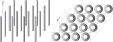
\includegraphics[width=0.8\textwidth]{Fundamentos/pendry.pdf}
	\caption{Metamateriales propuestos por Pendry. A la izquierda, un WSM (\textit{Wire Screen Medium}), que posee $\epsilon<0$ y $\mu>0$ cuando el campo eléctrico es longitudinal a los cables, para un rango de frecuencias determinado. A la derecha, un medio de SRR, que posee $\epsilon>0$ y $\mu<0$ cuando el campo magnético es perpendicular al eje de los anillos, para una frecuencia determinada \cite{Caloz:ElectromagneticMetamaterials}.}
	\label{fig:Pendry}
\end{figure}

\begin{figure}[htp]
	\centering
	\includegraphics[width=0.8\textwidth]{Fundamentos/metamateriales-smith.pdf}
	\caption{Estructuras metamateriales propuestas por Smith \cite{Caloz:ElectromagneticMetamaterials}.}
	\label{fig:metamaterial-de-smith}
\end{figure}

En el contexto de una línea de investigación, en principio, independiente de los trabajos previos de Veselago, la primera descripción de estructuras dieléctricas periódicas con una banda prohibida completa fue dada, en 1990, por Ho, Chan y Soukoulis, en Iowa, Estados Unidos, quienes propusieron un arreglo periódico de esferas dieléctricas, dispuestas en forma de capas. Para un rango amplio de radios de esferas, el efecto de banda prohibida se daba en todas direcciones. Posteriormente, Yablonovitch divisó una estructura cristalina simétrica de más fácil fabricación, que consistía en la producción de tres agujeros cilíndricos en un prisma dieléctrico, repetido periódicamente. Demostró, además, usando dichas estructuras, que la existencia de una banda prohibida electromagnética podía ser predicha teóricamente, en base, principalmente, a la constante de periodicidad del dieléctrico artificial.

Los trabajos de Yablonovitch, en estructuras de banda prohibida electromagnética, y Pendry, en metamateriales de índice de refracción negativo, se hicieron sobre estructuras con banda de interés en microondas, pero bajo modelos fotónicos, gracias a la linealidad de las ecuaciones de Maxwell. Esto permitió el uso de distintas técnicas conocidas y desarrolladas durante el siglo XX en microondas para el diseño de materiales fotónicos de estas características a partir de finales de la década de 1990, principalmente en ámbitos de investigación de ciencias básicas.

Al mismo tiempo, comenzaron los estudios sobre las denominadas "superficies electromagnéticas" (\textit{electromagnetic surfaces}), que consisten en superficies texturadas, generalmente conductoras (en contraposición a los trabajos tridimensionales) que imponen condiciones de contorno particulares, capaces de lograr cambiar la polarización de una onda incidente, influir sobre las ondas de superficie y controlar la fase de reflexión, actuando como estructras de banda electromagnética bidimensionales. La más simple consiste en una placa metálica coarrugada, como la mostrada en la figura \ref{fig:superficie-coarrugada}, de forma que las variaciones de altura sean de $\lambda/4$, que puede comportarse como una "superficie blanda" (\textit{soft surface}) o una "superficie dura" (\textit{hard surface}), en función de la polarización de la onda que se propaga \footnote{Si el campo eléctrico es perpendicular a las ranuras, la hendidura de profundidad $\lambda/4$ actúa como una línea de transmisión de cuarto de onda cortocircuitada, lo que, en la parte superior de las ranuras, se convierte en un circuito abierto, actuando como una superficie de alta impedancia. Si, en cambio, el campo eléctrico es paralelo a las ranuras, la impedancia que presenta es baja.}. Los primeros trabajos sobre estructuras bidimensionales con comportamiento de banda prohibida electromagnética dieron lugar a las denominadas FSS (Frequency Selective Surfaces, superficies selectoras de frecuencias) \cite{Munk}. En 1999, Sievenpiper \cite{Sievenpiper:Thesis} propuso, en su tesis doctoral, estructuras superficiales compactas de alta impedancia, de manera que no fuera necesario el uso de una distancia de $\lambda/4$ entre la superficie superior y la inferior para lograr el efecto deseado, dado que se cargaba capacitivamente a la estructura \cite{Marcela:Tesis} \cite{Sievenpiper:HIESForbiddenBand}. Estas nuevas estructuras periódicas consisten en un arreglo metalodieléctrico de subestructuras denominadas "hongos" (\textit{mushrooms}), como se muestra en la figura \ref{fig:sievenpiper}, y proveen condiciones de borde de alta impedancia para polarizaciones TE y TM al mismo tiempo.

\begin{figure}[H]
	\centering 
	\subfigure[Superficie coarrugada tradicional]{
		\label{fig:superficie-coarrugada}
		\includegraphics[width=0.35\textwidth]{Fundamentos/superficie-coarrugada.pdf}}
	\hspace{30pt}
	\subfigure[Superficie propuesta por Sievenpiper \cite{Sievenpiper:Thesis}]{
		\label{fig:sievenpiper}
		\includegraphics[width=0.45\textwidth]{Fundamentos/sievenpiper.pdf}}
	\caption{Superficie coarrugada tradicional para lograr superficies blandas y duras, y superficie propuesta por Sievenpiper.}
	\label{fig:sievenpiper-comparacion}
\end{figure}

El principal interés práctico de las estructuras propuestas por Sievenpiper radica en que actúan como conductores magnéticos artificiales, es decir, tienen una fase de reflexión nula para ondas incidentes, al mismo tiempo que presentan una banda prohibida electromagnética para las ondas de superficie. Esto se puede explicar a baja frecuencia considerando un modelo cuasiestático, dado que la distancia entre los parches conductores de la capa superior dan lugar, debido a la distancia que los separa, a una capacidad. La corriente que circula entre parches vecinos por efecto de una onda de superficie da lugar, análogamente, a una inductancia. Cuando el circuito resonante paralelo que forman resuena, la impedancia aumenta, dando lugar a una banda prohibida. Para frecuencias menores a la de resonancia, la superficie es inductiva y soporta ondas TM, mientras que para frecuencias mayores a la misma, la superficie es capacitiva, lo que permite la existencia de ondas TE. La explicación para las bandas prohibidas en mayores frecuencias requiere un análisis de redes y campos.

En base a la propuesta de Sievenpiper, y en búsqueda de una mayor facilidad de fabricación, en 2001 Yang propuso la aplicación de los conceptos de superficies selectoras de frecuencias (FSS) con la intención de lograr un comportamiento similar, pero evitando el uso de vías entre el plano conductor inferior y las estructuras ubicadas en la segunda capa. Estas nuevas estructuras uniplanares son de más fácil fabricación, reduciendo al mismo tiempo el costo, aunque los anchos de banda prohibida electromagnética para ondas de superficie se redujeron ampliamente. El bajo costo, el bajo peso y el bajo perfil de estras estructuras las volvieron de particulares interés en el diseño de antenas.



%\section{Difracción de Bragg}
%\label{sec_bragg}
%%%%%
%% Caloz, pag 19
%% Kamgaing (tesis), pagina22
%\lipsum

\section{Teorema de Bloch-Floquet}

El teorema Floquet fue presentado por Gaston Floquet en 1883, y explicita la forma canónica de las soluciones a ecuaciones diferenciales lineales ordinarias de coeficientes periódicos de la forma $x' = A(t)x$, con $t \in \Re$, $X \in \Re^n$, donde $A(t)$ es una función periódica con periodo $p$. Si $x=\phi(t)$ es solución, entonces también lo es $x=\phi(x\pm np)$, con $n \in \mathbb{N}$. Esto significa que toda solución encontrada para el sistema con condiciones de contorno periódicas, es también periódica, con la misma periodicidad que las condiciones de borde. Un resultado análogo en física del estado sólido es el teorema de Bloch, que indica que las soluciones a la función de onda de un electrón en un cristal tiene la forma:

\begin{equation}
\phi(\vec{r}) = e^{j\vec{k} \cdot \vec{r}} u(\vec{r})
\end{equation}

donde $\vec{k}$ es el vector de onda cristalino, $\vec{r}$ es la posición y $u(\vec{r})$ es una función periódica con igual periodicidad que el cristal.

La idea intuitiva detrás del resultado radica en que si la estructura es infinitamente periódica, con celdas unitarias idénticas, las mismas deberían ser indistinguibles, por lo que los campos electromagnéticos deberían repetirse, a excepción de un corrimiento de fase. Por lo tanto, se puede escribir:

\begin{equation}
	E(x,y,z+d) = e^{j \beta d} E(x,y,z)
\end{equation}

donde $\beta$ es la constante de propagación en el medio periódico \cite{TaylorandFrancis}. El valor de la diferencia entre los campos en dos bordes de una celda unitaria, entonces, es $\beta d$, que puede reducirse al rango $[-\pi,\pi]$, de modo que los posibles valores de $\beta$ son $[-\pi/d,\pi/d]$, denominada la zona de Brillouin unidimensional. Todos los restantes valores de número de onda relevantes a la propagación dentro de la estructura periódica pueden ser reducidos a valores dentro de la Zona de Brillouin, ya que la misma contiene todos los número de onda físicamente posibles dentro de una estructura periódica.

% EN ALGUN MOMENTO HAY QUE HABLAR DE LA ZONA DE BRILLOUIN PARA MÁS DIMENSIONES, Y HAY QUE HILAR CON LA RELACIÓN DE DISPERSIÓN, QUE TAMBIÉN ES PERIÓDICA.
\section{Relación de dispersión}
\label{sec_bloch}
%%%%
% Libro de rahmat. Pagina 46.
% Zona de brillouin. Rahmat, libro, pagina 31.
% Diagrama de dispersión. Página 67 Rahmat. Caloz: pagina 106.
% Impedancia de Bloch: Caloz, pagina 113
% Tesis Choi, pag 82.
% Tesis Kovacs, pag 13.
% Venkateswaran, pag 26.
% Tesis Zheng, pag 5-8

Las estructuras periódicas se usan comunmente en microondas, principalmente como filtros, dado que pueden ser modeladas como líneas de transmisión cargadas, lo que permite describir las características que comparten con los mismos, utilizando nomenclaturas similares para fenónemos similares.

Una línea de transmisión infinita cargada periódicamente puede analizarse planteando las matrices ABCD\footnote{Las matrices ABCD son matrices que relacionan la corriente y la tensión a la entrada con la corriente y la tensión a la salida de un sistema. De esta manera, los parámetros A y D son adimensionales, el parámetro B tiene dimensiones de impedancia, y el parámetro C tiene dimensiones de admitancia.} de cada celda unitaria, considerando puntual el efecto de carga que impone la geometría, de forma que:

\begin{equation}
	\begin{bmatrix}
		V_n \\
		I_n
	\end{bmatrix}
	=
	\begin{bmatrix}
		A & B \\
		C & D
	\end{bmatrix}
	\begin{bmatrix}
		V_{n+1} \\
		I_{n+1}
	\end{bmatrix}
\end{equation}

Si se considera que la línea está cargada con una impedancia y una admitancia, como indica la figura \ref{fig:linea-transm-cargada-periodica}, entonces se puede dividir a cada celda unitaria en secciones diferenciadas, y multiplicar las matrices $\text{ABCD}_{i}$ de cada sección para obtener la matriz ABCD que corresponde a la celda unitaria completa;

\begin{enumerate}
	\item La primera mitad de la línea de transmisión, de largo $d/2$, cuya matriz ABCD es, considernado $Z_0$ su impedancia característica y $\beta_{TL}$ la constante de propagación \cite{Pozar:MwEngineering}:
	\begin{equation}
		\begin{bmatrix}
			A & B \\
			C & D
		\end{bmatrix}_{1,3}
		=
		\begin{bmatrix}
			\cos(\beta_{TL} d/2) & j Z_0 \sin(\beta_{TL} d/2) \\
			j Y_0 \sin(\beta_{TL} d/2) & \cos(\beta_{TL} d/2)
		\end{bmatrix}
	\end{equation}
	\item La carga, que comprende a la impedancia $Z$ y la admitancia $Y$ asociada a la línea de transmisión. La matriz resulta:
	\begin{equation}
		\begin{bmatrix}
			A & B \\
			C & D
		\end{bmatrix}_{2}
		=
		\begin{bmatrix}
			1+ZY & Z \\
			Y & 1
		\end{bmatrix}
	\end{equation}
	\item La segunda mitad de la línea de transmisión, de largo $d/2$, de igual expresión que la primera mitad.
\end{enumerate}

Si se considera que la relación entre las tensiones y corrientes de entrada y salida, respectivamente, están relacionadas por el factor de propagación $e^{-\gamma d}$, donde $\gamma$ es el módulo del vector de onda en el medio metamaterial que se quiere obtener, entonces:

\begin{equation}
	\begin{bmatrix}
		V_n \\ I_n
	\end{bmatrix}
	=
	\begin{bmatrix}
	A & B \\
	C & D
	\end{bmatrix}
	\begin{bmatrix}
	V_{n+1} \\
	I_{n+1}
	\end{bmatrix}
	=
	\begin{bmatrix}
	V_{n+1}e^{\gamma d} \\ 
	I_{n+1}e^{\gamma d}
	\end{bmatrix}
	\implies
	\begin{bmatrix}
	A-e^{\gamma d} & B \\
	C & D-e^{\gamma d}
	\end{bmatrix}
	\begin{bmatrix}
	V_{n+1} \\ I_{n+1}
	\end{bmatrix}
	= 0
\end{equation}

La existencia de una solución no trivial del sistema de ecuaciones planteado requiere que el determinante de la matriz se anule. Recordando, además, que en las redes recíprocas, $AD-BC=1$ \cite{Pozar:MwEngineering}:

\begin{subequations}
	\begin{align}
		AD + e^{2 \gamma d} - (A+D)e^{\gamma d}-BC = 0 \implies &1+e^{2\gamma d}-(A+D)e^{\gamma d} = 0 \\
		&\cosh (\gamma d) = \frac{A+D}{2}
	\end{align}
\end{subequations}

Reemplazando los valores de A y D de la matriz de transmisión de la celda unitaria completa, que surge de la multiplicación de las matrices de transmisión que la componen:

\begin{equation}
\cosh (\gamma d) = \frac{Y Z}{2} \cos{\left (\beta_{TL} d \right )} + \frac{i Y Z_{0}}{2} \sin{\left (\beta_{TL} d \right )} + \frac{i Z}{2 Z_{0}} \sin{\left (\beta_{TL} d \right )} + \cos{\left (\beta_{TL} d \right )}
\end{equation}

Dado que $\gamma = \alpha + j \beta$ es la constante de onda en el material, resulta conveniente considerar el caso en que no hay comportamientos exponenciales negativos para las ondas que los atraviezan, de modo que $\alpha=0$ \footnote{$\cosh (\gamma d) = \cosh(\alpha d)\cos(\beta d) + j \sinh(\alpha d) \sin(\beta d) = \cos (\beta d)$}. Se obtiene, entonces, la ecuación de dispersión para una dimensión:

\begin{align}
	cos(\beta d) = \frac{Y Z}{2} \cos{\left (\beta_{TL} d \right )} + \frac{i Y Z_{0}}{2} \sin{\left (\beta_{TL} d \right )} + \frac{i Z}{2 Z_{0}} \sin{\left (\beta_{TL} d \right )} + \cos{\left (\beta_{TL} d \right )}
\end{align}

\section{Impedancia de onda y de superficie}
\label{sec_imp_superficie}
%%%%
% Rahmat. Pagina 77 libro.
% Engheta, pagina 290.
\lipsum

%%%%
\lipsum
% Lightline stuff. Rahmat, pagina 28. Caloz, pagina 139. Pozar pag 386
\section{Tipos de EBG}
\label{sec_tipos_mtm}
%%%%
\lipsum[1]
% Tesis de kovacs, pagina 7.
\subsection{EBGs uniplanares}
\label{subsec_ebg_uniplanar}
%%%%
\lipsum
% buena intro en rahmat (libro), pagina 35-37
% Buscar las distintas formas, incluyendo Peano. Relación con FSS.
% Buena intro esn Goussetis, Feresidis, Vardaxoglou.
% Diseños para incidencia obliucua: Kim, Yand, Elsherbeni. Tambien en Lin, Li, Zhang.
% Hilbert: McVAy, Engheta, Hoorfar.
% Power loss analysis: Mohajer-Iravani, Ramahi, de Hindawi corp.
% Kern, Douglas, Werner.
% Analisis en Goussetis, Feresidis, paper posta. Tipos de resonancia.
% Lamminen, Vimpari, Saily. 
% Maci, Caiazzo, Cucini. Jodido, interesante. Leer.
\section{Modelado y simulación de metamateriales}
\label{sec_simulacion_mtm}
%%%%
\lipsum
% Un modelado medio simple se puede ver en la tesis de Choi, pag 90-99
\subsection{Métodos de cavidades periódicas}
\label{subsec_eigenfunctions}
%%%%
\lipsum
% Fullwave: Baccarello, Paulotto, impreso.
% Hacer estudio gráfico similar al CALOZ, pag 176.
\subsection{Modelado por líneas de transmisión}
%%%%
\lipsum
% Caloz, pag 60, 67, 76, 79
% Bidimensional, Caloz, pag 133
% Rahman Stuchly.ç
% Calculo de la inductancia de meander inductors: Stojanovic, Zivanov
% Cuentas! Wu, Lin, Wang, Wang, Chen
% Kim, Schutt-Ainé, 178. Modelado para PDN.
%Venkateswaran, pag 40 en adelante.
% Impedancia: hacer algo similar. Tesis Zheng, pag 8

\subsubsection{TMM}
%%%%
\lipsum[2]
% Caloz, pagina 144
% Choi (tesis), pag 54
\subsubsection{TLM}
\label{subsubsec_tlm}
%%%%
\lipsum
% Caloz, pag 155